\documentclass[11pt]{standalone}
\usepackage{amssymb}
\usepackage{amsmath}
\usepackage[no-math]{fontspec}
\usepackage{unicode-math}
\usepackage{libertinus}
\usepackage{pgf,xcolor}
\usepackage{tikz}
\usetikzlibrary{arrows.meta, backgrounds, decorations.pathreplacing, calc}
\usepackage{pgfplots}
\pgfplotsset{compat=newest}

\definecolor{my_darkgray}{HTML}{484949}
\definecolor{my_lightgray}{HTML}{F3F4F4}
\definecolor{my_darkblue}{HTML}{005A94}
\definecolor{my_lightblue}{HTML}{CCDEE9}
\definecolor{my_yellow}{HTML}{FFEC7F}
\definecolor{my_red}{HTML}{E60000}
\definecolor{my_orange}{HTML}{E87846}

\begin{document}
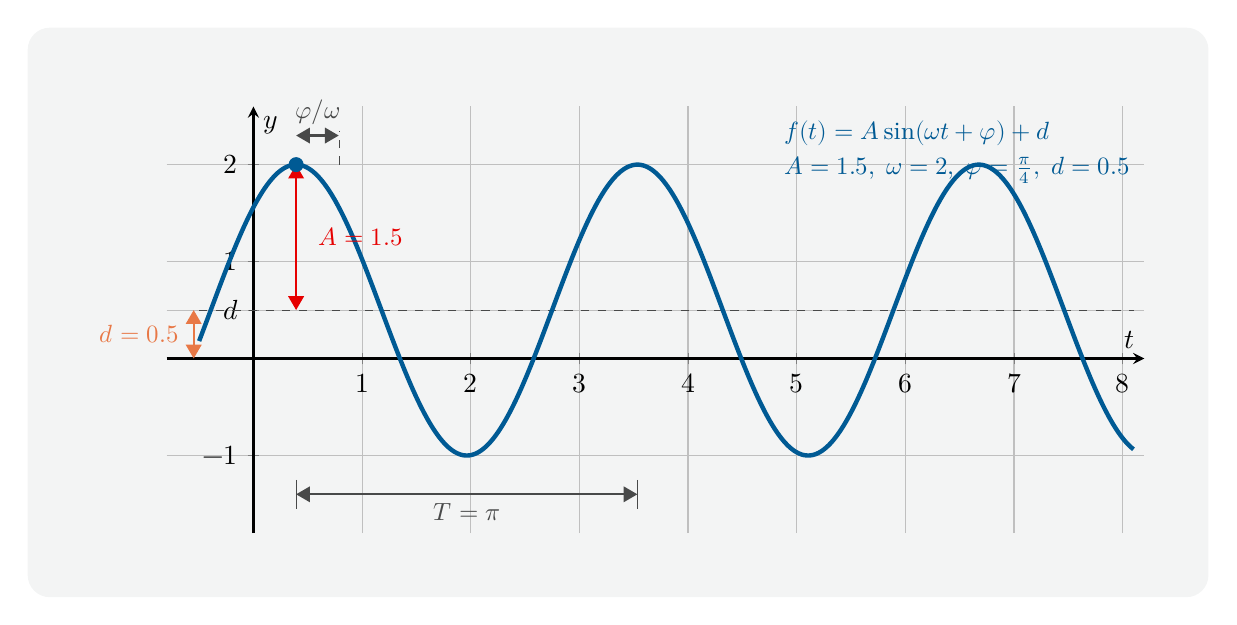
\begin{tikzpicture}[
    show background rectangle,
    background rectangle/.style={fill=my_lightgray, rounded corners=8pt},
    inner frame sep=0.8cm
]

% Parameters: A=1.5, omega=2, phi=pi/4, d=0.5
%   f(t) = 1.5 * sin(2t + pi/4) + 0.5
%   Period T = 2*pi/omega = pi ≈ 3.1416
%   Amplitude A = 1.5  →  range: d - A = -1 to d + A = 2
%   Vertical offset d = 0.5
%   Phase shift: first maximum at 2t + pi/4 = pi/2  →  t = pi/8 ≈ 0.393
%   Zero crossing (rising) at 2t + pi/4 = 0  →  t = -pi/8 ≈ -0.393

\begin{axis}[
    axis lines=center,
    xlabel={$t$},
    ylabel={$y$},
    height=7cm, width=14cm,
    xmin=-0.8, xmax=8.2,
    ymin=-1.8, ymax=2.6,
    xtick={0, 1, 2, 3, 4, 5, 6, 7, 8},
    ytick={-1, 0, 0.5, 1, 2},
    yticklabels={$-1$, $0$, $d$, $1$, $2$},
    grid=both,
    axis line style={thick},
    clip=false,
]

% ── Center line (vertical offset d = 0.5) ────────────────────────────────────
\addplot[draw=my_darkgray, dashed, thin, domain=-0.5:8.1]{0.5};

% ── Main sinusoidal curve: f(t) = 1.5*sin(2t + pi/4) + 0.5 ──────────────────
\addplot[draw=my_darkblue, samples=500, ultra thick, domain=-0.5:8.1]
    {1.5*sin(deg(2*x + pi/4)) + 0.5};

% ── First maximum: 2t + pi/4 = pi/2  →  t = pi/8 ≈ 0.3927 ───────────────────
\pgfmathsetmacro{\tmax}{pi/8}
\addplot[only marks, mark=*, mark size=2.5pt, draw=my_darkblue, fill=my_darkblue]
    coordinates{(\tmax, 2)};

% ── Amplitude annotation (double-headed arrow, my_red) ───────────────────────
% Arrow from center line (d=0.5) up to maximum (y=2) at t = t_max
\draw[{Triangle[length=5pt]}-{Triangle[length=5pt]}, my_red, thick]
    (axis cs:\tmax, 0.5) -- (axis cs:\tmax, 2.0);
\node[right, font=\small, my_red] at (axis cs:{\tmax + 0.12}, 1.25)
    {$A = 1.5$};

% ── Period annotation (double-headed arrow below the curve, my_darkgray) ─────
% One period from first max (pi/8) to next max (pi/8 + pi)
\pgfmathsetmacro{\tmaxnext}{\tmax + pi}
% Arrow sits at y = -1.4
\draw[{Triangle[length=5pt]}-{Triangle[length=5pt]}, my_darkgray, thick]
    (axis cs:\tmax, -1.4) -- (axis cs:\tmaxnext, -1.4);
\node[below, font=\small, my_darkgray] at (axis cs:{(\tmax+\tmaxnext)/2}, -1.4)
    {$T = \pi$};
% Small vertical tick marks at the period endpoints
\draw[my_darkgray, thin]
    (axis cs:\tmax,    -1.25) -- (axis cs:\tmax,    -1.55);
\draw[my_darkgray, thin]
    (axis cs:\tmaxnext,-1.25) -- (axis cs:\tmaxnext,-1.55);

% ── Vertical offset annotation (brace on y-axis side, my_orange) ─────────────
% Brace from y=0 to y=d=0.5, placed left of the y-axis
\draw[{Triangle[length=5pt]}-{Triangle[length=5pt]}, my_orange, thick]
    (axis cs:-0.55, 0) -- (axis cs:-0.55, 0.5);
\node[left, font=\small, my_orange] at (axis cs:-0.6, 0.25)
    {$d = 0.5$};

% ── Phase shift annotation (my_darkgray, showing horizontal offset) ───────────
% The unshifted sin(2t) first crosses zero rising at t=0; our curve crosses
% at 2t + pi/4 = 0  →  t = -pi/8.
% We annotate the horizontal distance from t=0 to the first rising zero
% crossing of the shifted curve.  That crossing is at t = -pi/8 ≈ -0.393,
% which is left of the plot window. Instead we annotate the shift relative
% to the unshifted cosine peak:
% Unshifted sin(2t) max would be at t = pi/4; our curve max is at t = pi/8.
% Horizontal arrow from pi/8 to pi/4 at y = 2.3 (above the curve)
\pgfmathsetmacro{\tunshifted}{pi/4}
\draw[{Triangle[length=5pt]}-{Triangle[length=5pt]}, my_darkgray, thick]
    (axis cs:\tmax, 2.3) -- (axis cs:\tunshifted, 2.3);
\node[above, font=\small, my_darkgray]
    at (axis cs:{(\tmax+\tunshifted)/2}, 2.31)
    {$\varphi/\omega$};
% Reference tick at the unshifted maximum position
\draw[dashed, my_darkgray, very thin]
    (axis cs:\tunshifted, 2.0) -- (axis cs:\tunshifted, 2.35);

% ── Angular frequency label in the legend area ───────────────────────────────
\node[my_darkblue, font=\small, anchor=north west]
    at (axis cs:4.8, 2.55)
    {$f(t)=A\sin(\omega t + \varphi)+d$};
\node[my_darkblue, font=\small, anchor=north west]
    at (axis cs:4.8, 2.18)
    {$A=1.5,\;\omega=2,\;\varphi=\tfrac{\pi}{4},\;d=0.5$};

\end{axis}
\end{tikzpicture}
\end{document}
